% Use line with ``preprint'' to get double-spaced
% preprint version. Use line without preprint to get
% version to submit to PRE.

\documentclass[%
%reprint,
aps,
prl,
showpacs,
twocolumn,
% preprint,
]{revtex4}

\usepackage{graphicx}  % needed for figures
\usepackage{dcolumn}   % needed for some tables
\usepackage{bm}        % for math
\usepackage{amssymb}   % for math
\usepackage{amsmath}
\usepackage{CJK}
\usepackage{subfig} % for subfigures
%\usepackage[colorlinks=true,backref=true]{hyperref} 

%%% Units
\newcommand{\unit}[1]{\ensuremath{\, \mathrm{#1}}}



\begin{document}
\begin{CJK*}{UTF8}{}
\CJKfamily{bsmi}

\title{Sub-10 Hz dark resonance at the cesium clock frequency induced by an optical frequency comb laser}


\author{Tsung-Han Wu (吳宗翰)}
 \altaffiliation{Currently at the College of Optical Sciences, University of Arizona}
\author{Yan-Long Peng (彭彥龍)}
\author{Sheng-Hui Lu (呂聖輝)}
 \altaffiliation{Currently at the College of Optical Sciences, University of Arizona}
\author{Wang-Yau Cheng (鄭王曜)}
 \email{wycheng@gate.sinica.edu.tw}
\affiliation{Institute of Atomic and Molecular Sciences,
Academia Sinica, Taiwan, R.O.C.}


\date{\today}

% Max of 600 characters for PRL, Rapid Comm abstracts.
\begin{abstract}
We used an optical frequency comb to resolve a dark state of
exceptionally narrow linewidth (5.6\unit{Hz}) in cesium gas buffered
with neon atoms, by precisely controlling the comb repetition rate.
The substantial pressure shift of the clock frequency expected
from the literature CW measurements was not observed. We
used optical Bloch-equations to interpret the experimental results. The
reported resonance has potential not only to enhance the
frequency discrimination of a microwave clock to the sub-10~Hz level,
but also to provide a link from the microwave time standard to the
optical frequency.
\end{abstract}

\pacs{
%39.30.+w,  %% Does not exists! What was it?
32.70.Jz,  % Line shapes, widths, and shifts 
% 32.50.+d,   % Fluorescence, phosphorescence (including quenching)
32.80.Qk,    % Coherent control of atomic interactions with photons  
% 32.10.Fn    % Fine and hyperfine structure 
42.50.Gy,    % Effects of atomic coherence on propagation, absorption, and amplification of light; electromagnetically induced transparency and absorption 
% 42.62.Eh,    % Metrological applications; optical frequency synthesizers for precision spectroscopy 
% 42.62.Fi,    % Laser spectroscopy 
}

\maketitle
\end{CJK*}

Ultimate atomic wavefunction control needs resolution at hyperfine
level and needs highly coherent electromagnetic waves to build up 
stable quantum interference. Quantum interference established by an 
optical frequency comb laser was recently demonstrated to be a novel 
approach for the ultimate wavefunction control~\cite{Stowe2008}, 
although precise applications were not discussed. In this work, 
we observed a comb-laser-induced mixed quantum state, which is 
often called a ``dark state'' generated by coherent population 
trapping (CPT)~\cite{Vanier2005}. We also point out a potential clockwork 
application via direct transfer of the microwave frequency standard to an optical 
frequency. Comb-laser-based Cs CPT clock, once developed with a high 
Q-value ($\nu/\delta\nu$), would be generalizable to extremely wide-band
wavelength regions~\cite{Gohle2005, Dudley2006} due to the high peak power, and 
should therefore have much wider application than a CW-based CPT clock.
    
 Probing a dark resonance by a mode-locked pulse train was first demonstrated 
by Arissian and Diels~\cite{Arissian2006}, who resolved a dark state of 627 kHz
linewidth with hot Rb atoms. They concluded from a theoretical analysis that 
stabilizing the laser frequency was not necessary to prepare their dark state. 
We confirm their observations here using our unique comb laser 
system~\cite{Cheng2008}, which allows for directly monitoring and controlling 
the mode frequency $f_n$~\cite{Cheng2008,Cheng2007} without interrupting the 
repetition rate locking. However, we observed a 5 order of magnitude 
narrower CPT linewidth in 8.7 kPa Ne buffer gas and we found, somewhat 
surprisingly, that our narrow dark-state position was not 
sensitive to buffer-gas pressure in an optical-thick medium. We were also 
aware that their modeling was only applicable in some situations, e.g., when 
the spectral linewidth of the intermediate states is much larger than the 
repetition rate or the hyperfine splittings that three-level model could fairly 
cope with. 

\section{CPT signal measurement}

\begin{figure*}
  \centering
  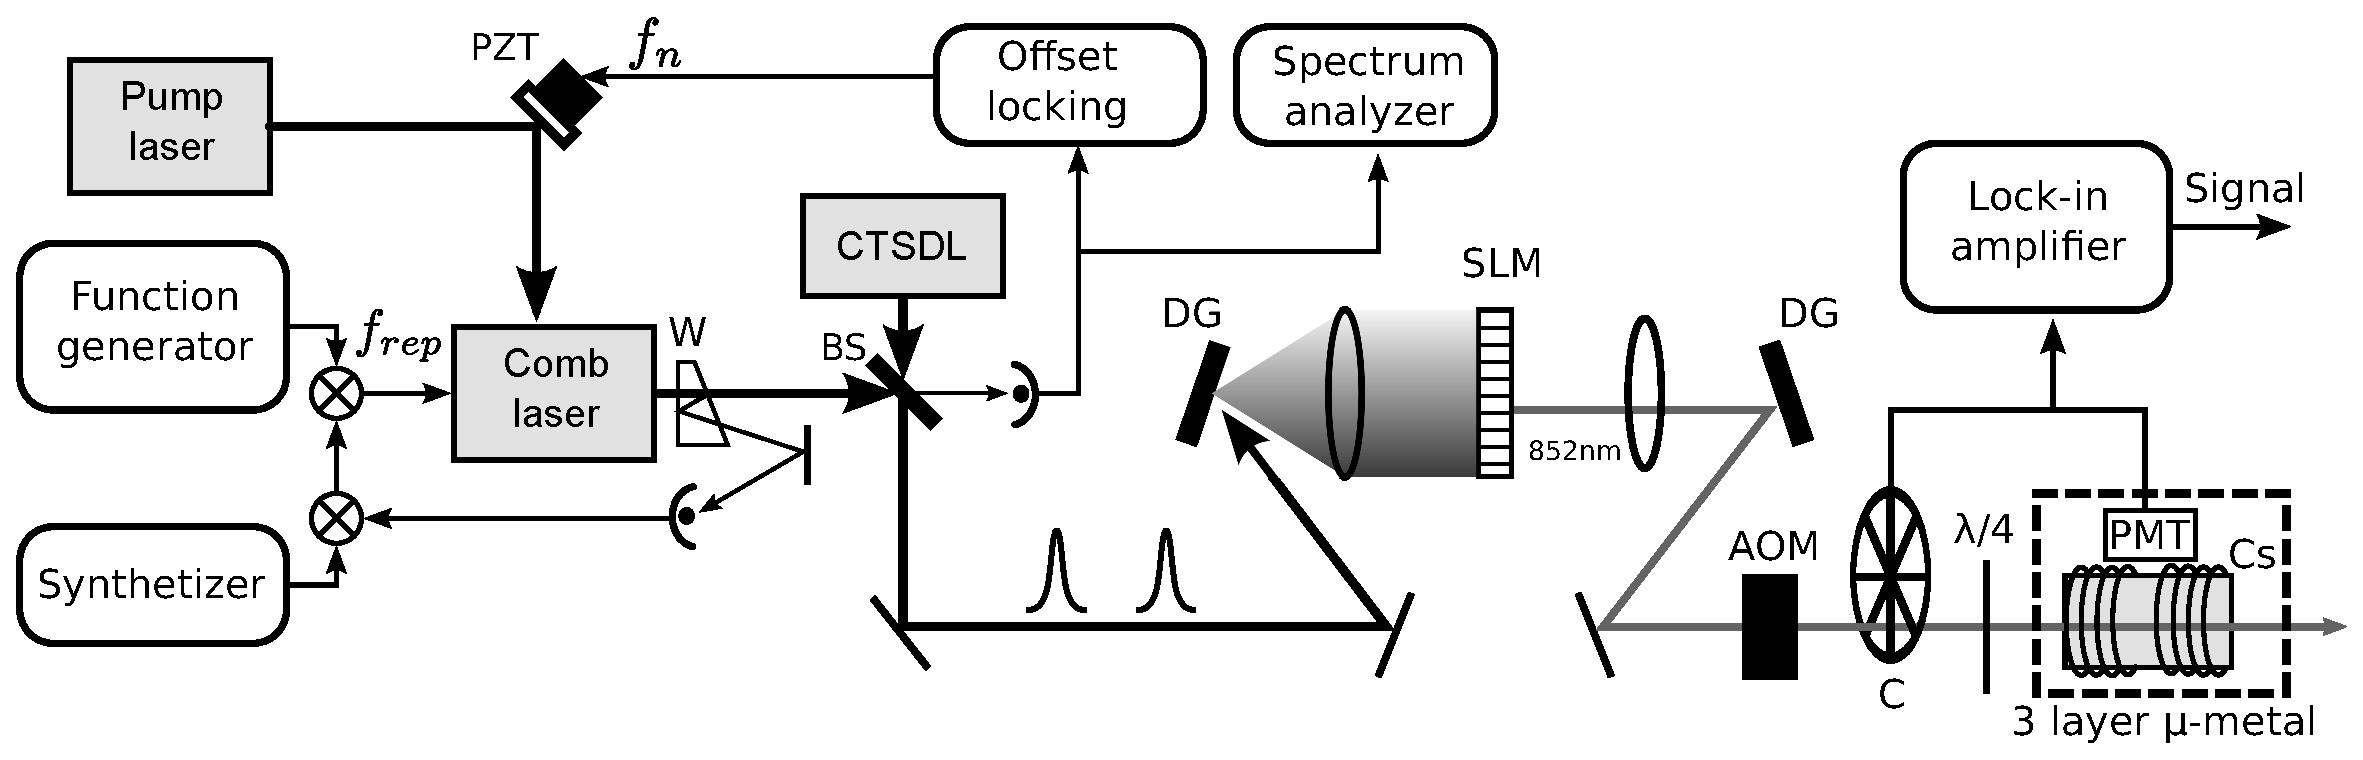
\includegraphics[scale=0.4]{experiment_big.eps}
  \caption{Experimental setup schematic. PZT: piezoelectric transducer; W: comb laser output wedge; CTSDL: cesium two-photon stabilized diode laser; BS: 70:30 beam splitter. The offset-locking circuit, the function generator and the synthetizer used a common timebase from a LORAN-C receiver. $f_n$ and $f_{rep}$ denotes the equipment that controls the mode frequency and the repetition rate, respectively. DG: diffraction grating; SML: spatial light modulator; AOM: acousto-optic modulator; C: chopper; $\lambda/4$: quarter-wave plate for 852 nm; PMT: photo-multiplier tube; Cs: cesium cell with buffer gas (see text for buffer types) and surrounding solenoid coil.}
  \label{fig:experiment}
\end{figure*}



To resolve the ultra-narrow dark resonance and to verify the role of mode 
frequency, we constructed a comb laser system [?] with the block diagram shown 
at the top of Fig. 1. The mode frequency was monitored by a reference laser 
whose frequency instability $\Delta f$ was 160 Hz in 60 second [?]. Mode-frequency $f_n$ 
locking was realized by horizontally shifting the pump beam with a piezoelectric 
transducer (PZT) [?]. The repetition rate $f_{rep}$ was phase locked against an 
synthesizer~ whose time base was referred to a satellite-based 5 MHz 
frequency standard via Loran-C. An additional [??] function generator was employed 
to improve the measurement resolution to 10~$\mu{\rm Hz}$. To ensure ``orthogonal control''
between the mode-frequency $f_n$ and the repetition rate $f_{rep}$, we dithered $f_n$ 
by the PZT indicated in Fig. 1, with the dither width ranging from 1 to 10 MHz, 
while simultaneously recording the maximum instability of the repetition rate 
locking. The result of this orthogonality inspection shows (inset of Fig. 1) 
that there is no correlation between frep and fn-dither-width at our 4-mHz measurement 
uncertainty. Here, as usual, $f_n$ and $f_{rep}$ are related by
\begin{equation*}
f_n = f_{rep}\left(n + \frac{\phi}{2\pi}\right)
\end{equation*}
where $n$ denotes the mode number and $\phi$ is the overall phase 
difference between successive pulses. The lower part of Fig. 1 shows the block 
diagram for retrieving the CPT signal. The 40 fs comb pulse, which was sent into
 the spatial light modulator (SLM) system, had 200 mW average power with a 
repetition rate of 91.92631770 MHz = (clock frequency)/100. The spatial light 
modulator extracted the 852 nm component from all other comb modes so the scattered 
background light from other wavelengths could be minimized. Consequently, 0.2 nm 
bandwidth comb modes with $140\pm0.05~\mu{\rm W/cm}^2$ average power were sent into a Cs cell, 
with a wrapping of three layers of $\mu$-metal and a solenoid coil on the inner 
shell of the $\mu$-metal. To reduce the spin-spin-exchange collisions as well as 
transit-time broadening~\cite{Hockel2009}, we tried different Cs vapor pressures and different 
buffer gases. A photomultiplier tube (PMT) detected fluorescence from
 Cs 6P$_{3/2}$~$\rightarrow$~6S$_{1/2}$ transition. The length of the light path from the input surface 
of the cell to the location of the PMT was 3.8 cm. The laser was chopped 
with 500 Hz and the small reduction of the flurescence was measured with a lock-in amplifier. An acousto-optical modulator (AOM) was used to 
stabilize the laser power to the noise level of $\pm 50$ nW. Power fluctuations at $\mu$W level will obscure the CPT signal.




\begin{figure}
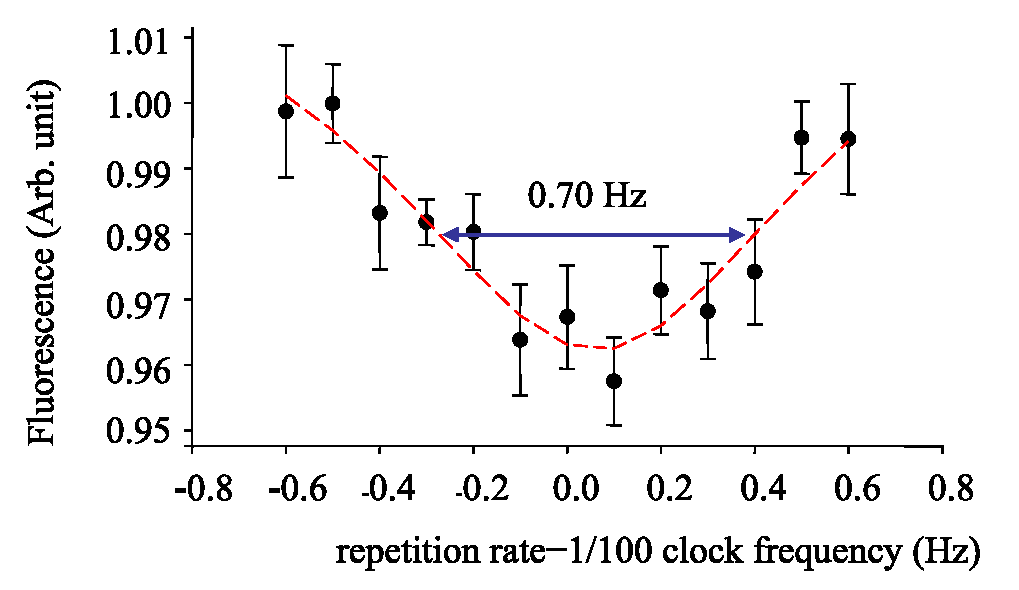
\includegraphics[scale=0.5]{cpt1_word}
\caption{\label{fig:cpt1} A figure caption. The figure captions are
automatically numbered.}
\end{figure}

% \begin{figure}
% 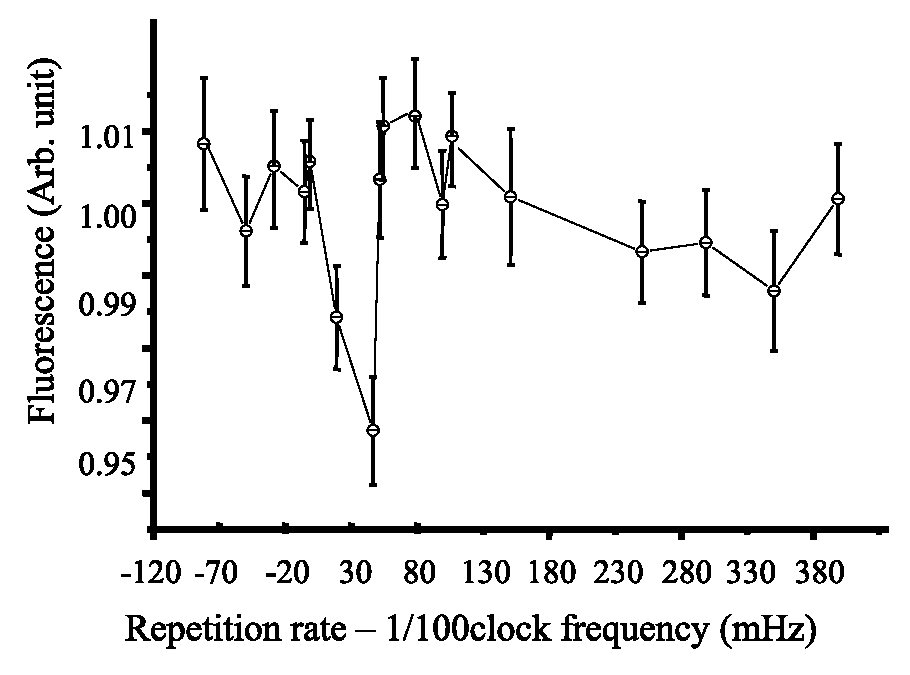
\includegraphics[scale=0.5]{cpt2_word}
% \caption{\label{fig:cpt2} A figure caption. The figure captions are
% automatically numbered.}
% \end{figure}

\begin{figure}
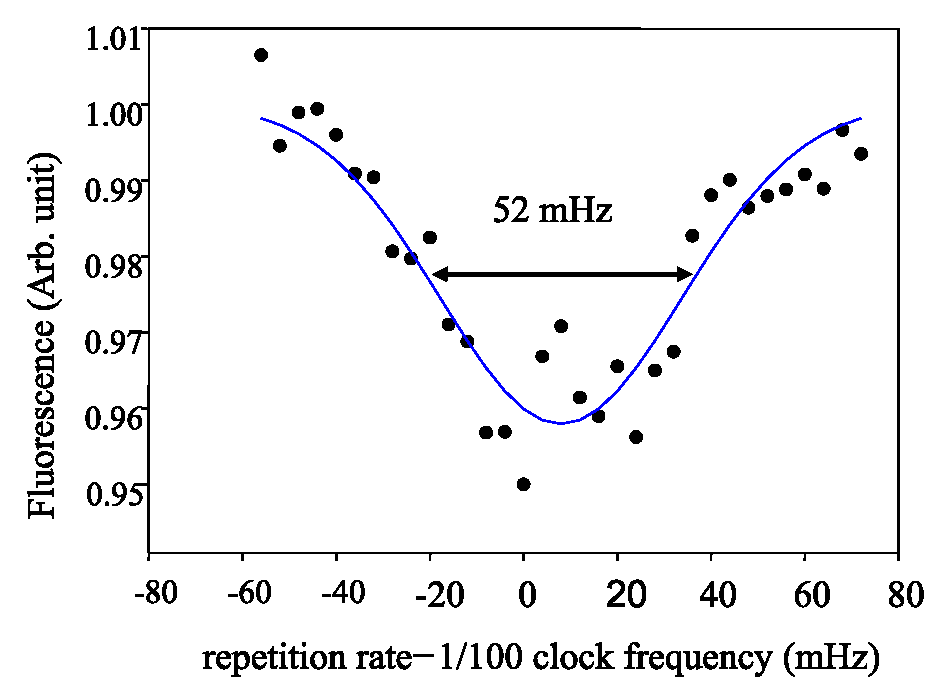
\includegraphics[scale=0.5]{cpt3_word}
\caption{\label{fig:cpt2better} A figure caption. The figure captions are
automatically numbered.}
\end{figure}

Fig. 2 shows experimental results for a mixed buffer gas of 1.5~kPa N$_2$ and 1.5~kPa He. Fig. 3 shows results for 8.7 kPa Ne buffer gas. In Figs. 2 and 3, the estimated spectral linewidth of a one-photon resonance ($\Delta \omega$) is 260~MHz and 750~MHz (D2 line), 
respectively, i.e., larger than the comb laser repetition rate (92~MHz). A CPT 
linewidth of 706~Hz (Gaussian fitting) with 4\% contrast was found at the laser 
repetition rate tuning over 1/100th of the clock frequency (Fig. 2). Sampling 
time for each data point was 30 seconds. Note that our Cs cell was heated to 
$100\pm0.001~^{\circ}{\rm C}$ to increase the optical density and was, therefore, no longer optically 
thin. We attribute the exceptionally narrow linewidth to the line-narrowing effect 
that occurs in an optically thick medium~\cite{Camparo1999, Knappe2001} and to the in-phase comb modes-atom 
interactions that leads to the reduction of FM-to-AM noise~\cite{Kao2005}. 

The narrowest CPT linewidth we measured was $5.2~\pm~0.6~{\rm Hz}$ (Fig. 3), which is 20-fold 
narrower than what has been achieved with a CW laser [?]. In Fig. 3, the 
scatter in the data points around the transparent dip is mainly due to the 
instrumental limitation [?] on the accuracy of repetition rate. Denser data 
points were obtained when a high resolution function generator [?] was employed, 
as shown in the inset of Fig. 3. By simultaneously monitoring the CPT-signal and
the mode-frequency, we found that the CPT signal was not sensitive to mode frequency, 
as the conclusion of Ref. 7. However, when the $f_n$ was dithered with a frequency faster 
than 10~kHz and a width larger than 1~MHz, the CPT signal could become indistinct, 
since severe FM-to-AM noise could be larger than the signal [??], though this situation did not in general occur in our well-controlled 
laser system. The interesting feature that a comb-laser based CPT signal depends on
 only one parameter, the repetition-rate, is encouraging news for 
simplifying any future repetition-rate based CPT standard. 

One puzzling phenomenon remains in this work, namely, no pressure shift was observed 
in our experiments, even though a pressure shift of 43 kHz was predicted under the 
conditions of 8.7~kPa Ne buffer gas at room temperature [??]. This lack of obvious pressure shift is more encouraging news for future 
CPT-clock devices.

\section{Theoretical calculation}

Since no theory has been reported on the subject of comb-laser-based CPT, we 
interpret our experimental results by employing a set of Bloch equations with 
density matrix elements similar to Ref. 2, except that the Rabi frequency changes 
rapidly with time, the dimension of the density matrix is extended to $4 \times 4$ for our 
four-level system, and Adomian's decomposition method [xiv] was adopted for solving 
the coupled partial differential equations in the time domain. To simplify the 
time-domain calculation, we let the pulse carrier frequency $f_c$ coincide with 
one comb mode $f_n$, and this simplification was examined and shown to have no 
influence on the conclusions of this letter. 

\begin{figure}
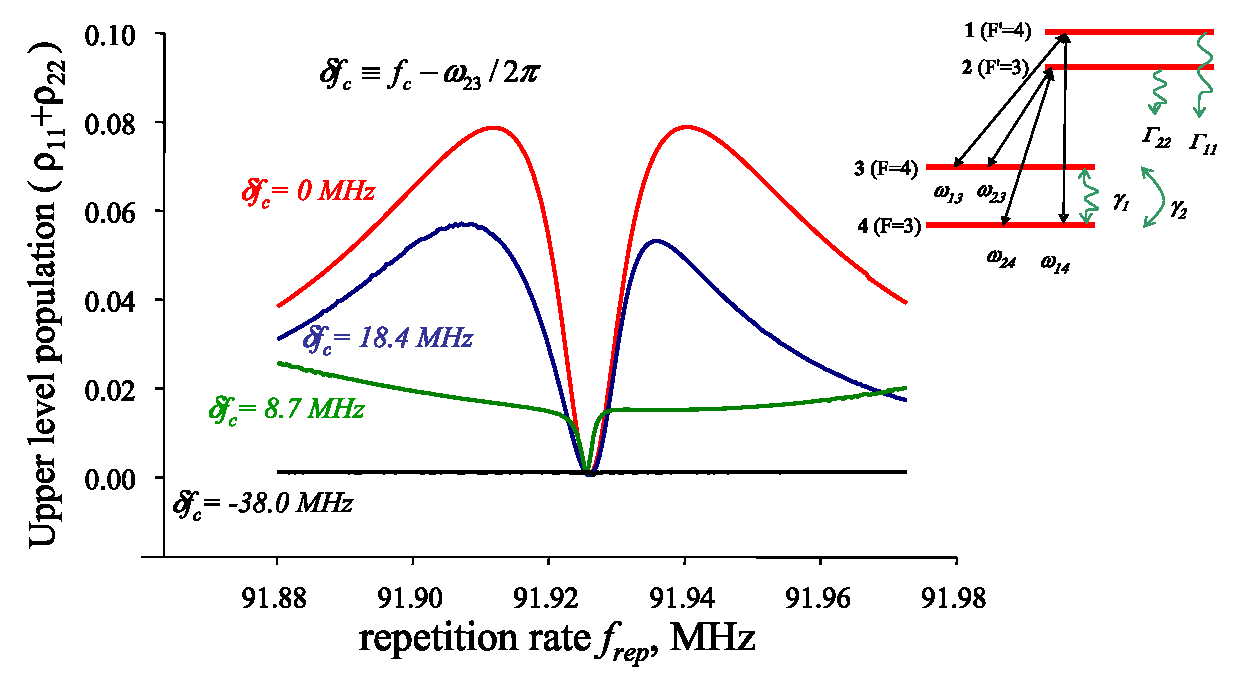
\includegraphics[scale=0.4]{theory1_word}
\caption{\label{fig:theory1} A figure caption. The figure captions are
automatically numbered.}
\end{figure}


\begin{figure}
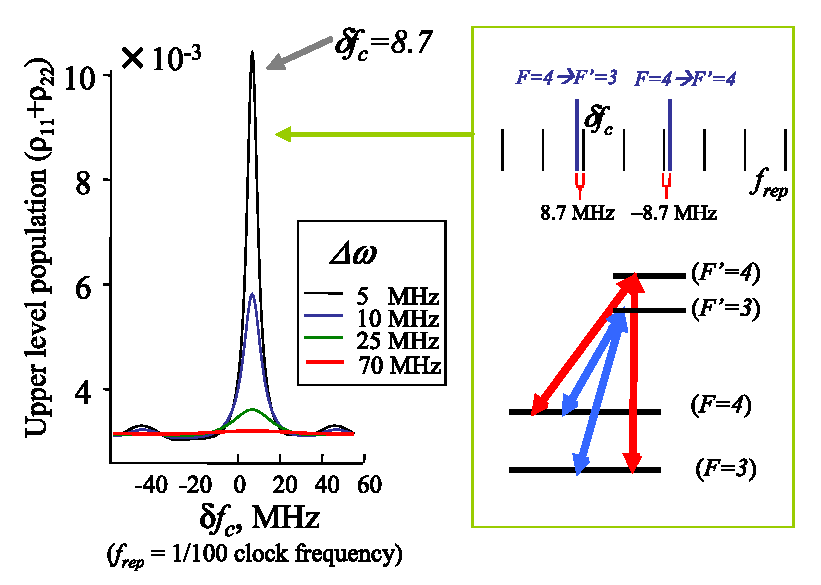
\includegraphics[scale=0.5]{theory2_word}% Here is how to import EPS art
\caption{\label{fig:wide}Use the figure* environment to get a wide
figure that spans the page in \texttt{twocolumn} formatting.}
\end{figure}


The corresponding level diagram is 
depicted on the right of Fig. 4 (a), where $\rho_{ij}$ denotes the matrix elements of the  density matrix, $\Gamma_{ij}$ is the level decay rate of excited states; $\gamma_1$, $\gamma_2$ 
are the decoherent rate of the diagonal and off-diagonal terms between level 3 and 4, 
respectively; and $\omega_{ij}$ is the level transition frequency between levels $i$ and $j$ ($i,j=1...4$). Note that,
$rho_{11}+\rho_{22}$, the total upper-level population, can be taken as the signature of ground 
state coherence when $\rho_{34}$ is built up. The level diagram in Fig. 4 (a) can be applied 
to both the D1 and D2 lines of the Cs atom. The other hyperfine levels of the D2 line,
namely, $F'=2$ and $F'=5$, are not relevant in building up the dark state, and are 
considered as part of the ground-state decoherence rate, i.e., as levels contributing 
to $\gamma_1$ and $\gamma_2$. All the data used in the simulation of this letter were taken from 
reference [?]. Fig. 4 shows that the CPT signal exhibits a carrier-frequency dependence, 
which is different from the conclusion in Ref. 7. The main cause of this difference 
is that the corresponding spectral width $\Delta \omega$ of the one-photon transitions is 
assumed as much smaller than the repetition rate, as in the case of a Cs MOT 
or atomic beam ($\Delta \omega = 5.2~{\rm MHz}$). In contrast, when the simulation is based on our experimental conditions in Fig. 3; that is, $\Delta \omega = 750~{\rm MHz}$; laser average power of
$140~\pm~0.05~\mu{\rm W/cm}^2$ and pulse width of 1 ps after the spatial light modulator, the 
CPT lineshape becomes insensitive to the carrier frequency of comb pulse, which 
is consistent with the conclusion in Ref. 5. Fig. 5 illustrates the concept of 
``arrier-frequency-dependent quantum interference'' as the frep in Fig. 4 is kept 
at 1/100th clock frequency. In other words, the ``bright bump'' indicated by the 
black curve of Fig. 5 shows an increase in ($\rho_{11}+\rho_{22}$). This interesting phenomenon cannot occur in a three-level system. Our interpretation is illustrated in the inset 
of Fig. 5: the two CPT channels, namely, $F=3 \leftrightarrow F'=3 \leftrightarrow F=4$ (blue path at the lower right) 
and $F=3 \leftrightarrow F'=4 \leftrightarrow F=4$ (red path at the lower right), can interfere with each other, 
which leads to a small ``bright bump'' in the dark state. The highest bump ($\delta f_c~=~8.7~{\rm MHz}$) 
happens when the comb laser carrier frequency is tuned such that the corresponding Rabi 
frequencies associated with the $F=4 \rightarrow F'=4$ and $F=4 \rightarrow F'=3$ transitions are the same but with 
opposite phase.  A similar situation happens for the other bump ($\delta f = -37.8~{\rm MHz}$). This 
$f_c$-dependent ``bright bump'' offers a chance to further stabilize the carrier frequency 
by locking.the repetition rate to the bump center, and thus the optical frequency is 
connected to microwave standard simply using a Cs cell.    

The authors are deeply indebted to Dr. Jyhpyng Wang for encouraging and kindly 
amending this article.  The author also thanks Dr. Ming-Sheng Chang, Dr. Ying-Chen Cheng, 
and Professor Jow-Tsong Shy for valuable comments, and Dr. Jon Hougen for the help 
with English corrections. We are grateful for the funding support of National 
Science Council in Taiwan with the project of NSC 94-2112-M-001-022-MY3.



\begin{thebibliography}{99}

\bibitem{Stowe2008} M.~C. Stowe, A. Pe'er and J. Ye, Phys. Rev. Lett. {\bf 100}, 203001 (2008).

\bibitem{Vanier2005} J. Vanier, Appl. Phys. B {\bf 81}, 421 (2005).

\bibitem{Gohle2005} C. Gohle, T. Udem, M. Herrmann, J. Rauschenberger, R. Holzwarth, H.~A. Schuessler, F. Krausz and T.~W. H\"{a}nsch, Nature {\bf 436}, 234 (2005).

\bibitem{Dudley2006} J.~M. Dudley, G. Genty and S. Coen, Rev. Mod. Phys. {\bf 78}, 1135 (2006).

\bibitem{Arissian2006} L. Arissian and J.-C. Diels, Opt. Comm. {\bf 264}, 169 (2006).

\bibitem{Cheng2008} W.-Y. Cheng, T.~H. Wu, S.~H. Huang S.~Y. Lin and C.~M. Wu, Appl. Phys. B {\bf 92}, 13 (2008).

\bibitem{Cheng2007} C.-Y. Cheng, C.~M. Wu, G.~B. Liao and W.~Y. Cheng, Opt. Lett. {\bf 32}, 536 (2007).

\bibitem{Synth} Agilent 8644A signal generator and Agilent 81150 function generator, respectively.

\bibitem{Camparo2007} J. Camparo, Phys. Today {\bf 60}, 33 (2007).

\bibitem{Lukin1997} M.~D. Lukin, M. Fleischhauer, A.~S. ibrov, H.~G. Robinson, V.~L. Velichansky, L. Hollberg and M. O. Scully, Phys. Rev. Lett. {\bf 79}, 2959 (1997).

\bibitem{Hockel2009} D. H\"{o}ckel, M. Scholz and O. Benson, Appl. Phys. B {\bf 94}, 429 (2009).

\bibitem{Camparo1999} J.~C. Camparo and J.~G. Coffer, Phys. Rev. A {\bf 59}, 728 (1999).

\bibitem{Knappe2001} S. Knappe, R. Wynands, J. Kitching, H.~G. Robinson and Leo Hollberg, JOSA B {\bf 18}, 1545 (2001).

\bibitem{Kao2005} Y.~M. Kao, T.~F. Jiang and I. A. Yu, Phys. Rev. E {\bf 72}, 066703 (2005).

\bibitem{Steck2009} D.~A. Steck, Cesium D line data, available online at http://steck.us/alkalidata (revision 2.1.2, 12 August 2009).

\end{thebibliography}



% \begin{figure}   % fig 1
% \caption{Density plot at time $t=500$ of the slow field
% $v(t,x,y)$ for a spatiotemporal chaotic state with
% $31$~spiral defects present. Dark and light regions
% correspond to values less or greater than the
% value~$v^*=0.484$ corresponding to the unstable fixed point;
% the field values span the range $v \in [0,a-b]$.  Parameter
% values were $\epsilon = 0.074$, $a = 0.84$, $b = 0.07$, $L =
% 50$, $\Delta{x} =0.5$ and~$\Delta t = 0.0037$. }
% \label{fig:pattern}
% \end{figure}

% \centerline{\epsfysize=3in \epsfbox{Pattern.eps}}


\end{document}
